\item \points{1b}
Follow the instructions in \texttt{src-linear/submission/logreg.py} to train a logistic regression classifier using Newton's Method. You will complete the |fit| and |predict| functions of the |LogisticRegression| class.

Starting with $\theta = \vec{0}$, run Newton's Method until the updates to $\theta$ are small: Specifically,  train until the first iteration $k$ such that $\vert\theta_{k} - \theta_{k-1}\vert_1 < \epsilon$, where $\epsilon = 1\times 10^{-5}$. Make sure to write your model's predicted probabilities on the validation set to the file specified in the code.

To verify a correct implementation, run the autograder test case |1b-4-basic| to create a plot of the \textbf{validation data} with $x_1$ on the horizontal axis and $x_2$ on the vertical axis. This plot uses a different symbol for examples $x^{(i)}$ with $y^{(i)} = 0$ than for those with $y^{(i)} = 1$. On the same figure, it will also plot the decision boundary found by logistic regression (i.e, line corresponding to $p(y\vert x) = 0.5$).

The output plot should look similar to the following (no plot submission is required): 

\begin{figure}[H]
	\centering
	\vspace{2mm}
	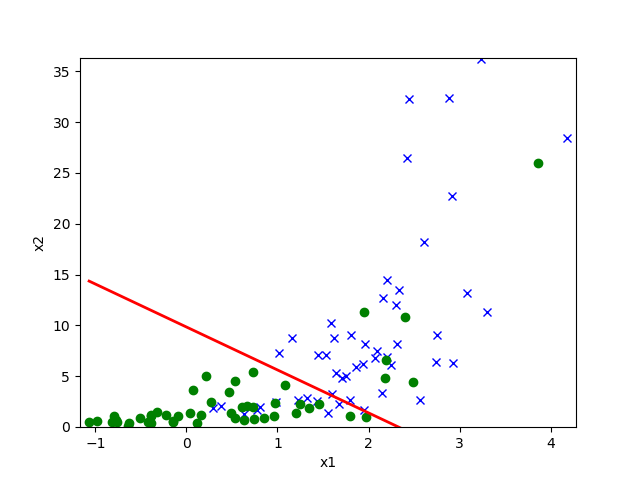
\includegraphics[width=0.65\linewidth]{01-linearclass/p01b_pred_1.png}
    \caption{Separating hyperplane for logistic regression on validation set of Dataset 1 (Note: This is for reference only.  You are not required to submit a plot.)}
\end{figure}
